\section{RQ1: How Often Do Approved Servers Change?}\label{sec:rq1}

We compare 33,130 consecutive version pairs across the 2,567 servers that yield comparable tools.\footnote{Four of the 2,571 servers expose ``tools'' only in evaluation or benchmark fixtures; once those are excluded they have nothing to compare.} Change is the norm. 1,814 servers (70.7\%) add at least one tool after their first tool-bearing release, and 1,687 (65.7\%) change the description of a tool that already existed. One in five version pairs (20.7\%) changes at least one existing description.

\paragraph{Capability gains}
Descriptions are what users read; capabilities are what code can do. 501 servers (19.5\%) have at least one existing tool that gains a capability class it did not have before, across 5,740 tool-level gain events. Gains are rarer per release than description edits: 2.6\% of version pairs contain one. Figure~\ref{fig:prevalence} breaks them down. Reading environment variables or secrets is the most common gain (289 servers, 11.3\%), followed by reading files (221, 8.6\%), writing or deleting files (171, 6.7\%), and network access (134, 5.2\%). Gaining the ability to run commands is less common but not rare: 75 servers (2.9\%) have a tool that could not run a program in one release and could in the next. Dynamically evaluated code is almost absent (13 servers).

\begin{figure}[t]
\centering
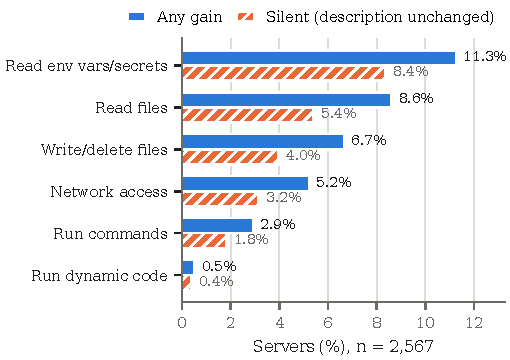
\includegraphics[width=\columnwidth]{figures/fig_prevalence.pdf}
\caption{Servers in which an existing tool gains each capability class (blue), and in which it does so while the tool's description stays byte-identical (orange, hatched). $n=2{,}567$ servers.}
\label{fig:prevalence}
\end{figure}

At the server level, where we look for each capability anywhere in the source rather than tracing it to a tool, 1,138 servers (44.3\%) gain at least one capability class over their history.

\paragraph{When gains happen}
Silent high-risk gains (Section~\ref{sec:rq2}) do not cluster at the start of a project, when a user might still be evaluating it. Among the 282 servers that have one, the median time from the first tool-bearing release to the first such gain is 43 days (interquartile range 9--126 days). A user who installed and approved the server in its first weeks would usually still be using the earlier approval when the capability arrives.

\paragraph{Releases versus commits}
A reader may worry that commit sampling (Section~\ref{sec:versions}) counts work in progress that no user installed. It does not inflate our results. Per version pair, silent capability gains occur at the same rate in the 1,584 servers we sampled at tagged releases and in the 983 we sampled at commits (12.8 per 100 pairs in both). Per server, tagged servers show more drift, 17.2\% with a silent gain against 8.4\%, because we observe more of their versions (a median of 15 against 5). The pooled server-level rates are therefore conservative for servers that publish releases, which are the versions users install.

\paragraph{New destinations}
1,391 servers (54.2\%) introduce at least one external hostname that did not appear in earlier versions. Most are documentation links or the APIs the server is built around; we use this signal only to locate changes in where data can go, not as evidence of misuse.

\begin{finding}{1}
Approved MCP servers change continually: two-thirds edit the descriptions users approved, and one in five gives an existing tool a new capability, typically weeks after release.
\end{finding}
